%% Based on a TeXnicCenter-Template by Gyorgy SZEIDL.
%%%%%%%%%%%%%%%%%%%%%%%%%%%%%%%%%%%%%%%%%%%%%%%%%%%%%%%%%%%%%

%----------------------------------------------------------
%
\documentclass[a4paper,12pt,reqno]{book}%
%
%----------------------------------------------------------
% This is a sample document for the AMS LaTeX Book or Monograph Class
% Class options
%       --  Body text point size:
%                        8pt, 9pt, 10pt (default), 11pt, 12pt
%       --  Paper size:  letterpaper (8.5x11 inch, default), a4paper
%       --  Orientation: portrait(default), landscape
%       --  Print side:  oneside, twoside (default)
%       --  Quality:     final(default), draft
%       --  Title page:  titlepage, notitlepage
%       --  Start chapter on left:
%                        openright (no, default), openany
%       --  Columns:     onecolumn (default), twocolumn
%       --  Omit extra math features:
%                        nomath
%       --  AMS fonts (noamasfonts available):
%                        noamsfonts
%       --  PSAMSfonts (fewer AMSfontsizes)
%                        psamsfonts
%       --  Equation numbering (equation numbers on the left is the default)
%                        leqno (default), reqno
%       --  Equation centering (equations centered is the default)
%                        centeredtags (default}, tbtags (top, bottom)
%       --  Displayed equations (centered is the default)
%                        fleqn (flush left)
% For instance the command
%          \documentclass[a4paper,12p,reqno]{amsbook}
% ensures that the paper size is a4, fonts are typeset at the size 12p
% and the equation numbers are on the right side.
\usepackage{lscape}
\usepackage{amsmath}%
\usepackage{amsfonts}%
\usepackage{amssymb}%
\usepackage{graphicx}%
\usepackage{chngcntr}%
\usepackage{epsfig}%
\usepackage{multirow}%
\usepackage{longtable}%
\usepackage{listings}%
\usepackage[utf8]{inputenc}
\usepackage[OT4]{polski}
\usepackage[dvips]{color}%
%\usepackage[left=35mm, right=20mm, top=20mm, bottom=30mm]{geometry}%
\usepackage{geometry}%
\usepackage[titletoc]{appendix}%
\usepackage{raport}%
\usepackage{setspace}%d
 \usepackage{url}%
%----------------------------------------------------------
\onehalfspacing
\numberwithin{equation}{chapter}%
\counterwithout{figure}{section}%
\counterwithout{figure}{chapter}%
%\counterwithout{table}{section}%
%\counterwithout{table}{chapter}%
%-----------------------------------------------------------

%-----------------------------------------------------------
\title{Analiza strumieniowa w internecie rzeczy}
\newcommand{\ownYear}{2016/2017}
\author{Dominik Waśniowski}
\newcommand{\supervisor}{Dr inż. Janusz Granat}
\newcommand{\lcol}[1]{\multicolumn{1}{l}{#1}}
\newcommand{\lcolDash}[1]{\multicolumn{1}{l|}{#1}}
\newcommand{\ccol}[1]{\multicolumn{1}{c}{#1}}
\newcommand{\comma}{\mbox{,}}
%----------------------------------------------------------

\newcommand{\streszczenie}{
W dzisiejszych czasach komputery i inne urządzenia elektroniczne generują dziennie terabajty danych.
Klasyczne metody ich analizą niewystarczające.
Zarówno z powodu wolumenu danych jak i bardziej wymagających użytkowników,
chcących szybciej otrzymywać wyniki.
Jednym ze sposobów przetwarzania danych w takich sytuacjach jest analiza strumieniowa.
Rozwiązania takie cechują się małymi opóźnieniami,
dane przetwarzane są na bieżąco, praktycznie w czasie rzeczywistym.
W ramach niniejszej pracy sprawdzono możliwości współczesnych systemów do przetwarzania strumieniowego: Esper,
Apache Spark i Apache Storm, a następnie dla platformy Storm przygotowano strumieniowe wersje algorytmów Bayesa i ADWIN.
Algorytm ADWIN został opracowany z wykorzystaniem dwóch różnych testów.
Pierwszym opartym o wartości średnie oraz drugim wykorzystującym stosunek gęstości rozkładów prawdopodobieństwa.
Algorytmy przetestowano na danych wygenerowanych losowo i na rzeczywistych.
}

\newcommand{\streszczenieen}{\textbf{Title}: Stream analysis in Internet of Things.\\[3mm]
Modern computers and other electronic devices generate terabytes of data daily.
Classic methods of data analysis are nowadays insufficient,
because of a high volume of data and more demanding users.
In this study it has been examined whether modern stream analysis frameworks
may help in changepoint detection.
Using Apache Storm framework implemented a stream version of algorithms: Bayes Online and ADWIN.
Algorithm ADWIN used two type of test.
First was based on mean and variance,
second used density ratio measure.
Algorithm were tested on artificial data sets and real data sets.
}

\newcommand{\slowakluczowe}{analiza strumieniowa, internet rzeczy, IoT, storm, wykrywanie zmian, Apache Storm}
\newcommand{\slowakluczoween}{stream analysis, internet of things, IoT, storm, changepoint detection}

%-----------------------------------------------------------
\begin{document}
\frontmatter
\newgeometry{centering}
\frontpage
\restoregeometry
\makeabstracts
\tableofcontents
\mainmatter
\chapter{Wprowadzenie}
Szacuje się,
że obecnie w użyciu jest 2 mld komputerów,
10 mld telefonów komórkowych,
a do 2020 r. do sieci ma być podłączone 20 mld urządzeń (Gartner, Inc., 2015).
Urządzenia te będą zbierać dane,
przetwarzać je
bądź przekazywać dalej.
Dzięki temu ludzie będą mogli wiedzieć więcej na temat otaczającego świata,
szybciej reagować na zmiany
czy podejmować lepsze decyzje.
Ogromne ilości danych generowane w każdej sekundzie,
oraz wymagania użytkowników aby wyniki otrzymywać coraz szybciej,
najlepiej od razu,
powodują,
że obecne metody przetwarzania danych stają się niewystarczające.
Wśród rozwiązań pozwalających radzić sobie w takich sytuacjach
coraz większą popularność zyskuje przetwarzanie strumieniowe (\textit{stream analysis, data streaming}).

Rozwiązania oparte na przetwarzaniu strumieniowym charakteryzują się wysoką przepustowością,
krótkimi czasami odpowiedzi i odpornością na awarie.
Dane mogą pochodzić z różnych źródeł: czujniki, komputery, telefony.
Możliwe jest tworzenie i wykonywanie analiz w czasie rzeczywistym,
dane przetwarzane są na bieżąco,
bezpośrednio po ich otrzymaniu.

Jednym z zagadnień związanych z przetwarzaniem danych jest wykrywanie zmian (sytuacji nietypowych).
Przez lata powstało wiele prac starających się rozwiązać ten problem.
Większość z nich oparta jest na analizie całościowej,
tj. zestawy danych,
które poddane są analizie,
przygotowywane są wcześniej i nie ulegają zmianie w czasie.
Algorytmy nie są w stanie na bieżąco analizować napływających danych.

Tematem niniejszej pracy jest zagadnienie wykrywania zmian w przebiegach czasowych,
oparte na mechanizmach statystycznych.

Celem pracy jest stworzenie mechanizmów wykrywających sytuacje nietypowe
z wykorzystaniem technik analizy strumieniowej.
W ramach pracy zostały sprawdzone dostępne platformy streamingowe:
\begin{itemize}
  \item Esper,
  \item Apache Spark,
  \item Apache Storm
\end{itemize}
pod kątem przydatności.
Aby sprawdzić skuteczność analizy strumieniowej zostały zaimplementowane algorytmy Bayesa (\textit{Bayesian Online Changepoint Detection})
oraz ADWIN.
Algorytmy w ramach pracy zostały zaadaptowane do wersji strumieniowych oraz przygotowane pod kątem platformy Apache Storm.
Analiza skuteczności badanych algorytmów została przeprowadzona z wykorzystaniem danych wygenerowanych losowo jak i rzeczywistych.

Układ pracy jest następujący.
Rozdział drugi przybliża tematykę związaną z analizą strumieniową.
W tym samym rozdziale znajduję się także porównanie dostępnych platform.
W rozdziale trzecim przedstawiono teoretyczne aspekty związane z wykrywaniem zmian.
Rozdział czwarty z kolei dokładnie przedstawia wykorzystane algorytmy.
W rozdziale piątym znajdują się wyniki przeprowadzonych eksperymentów.
Ostatni rozdział stanowi podsumowanie.
W dodatku A znajduje spis zawartości płyty CD.


\chapter{Analiza strumieniowa}
\label{ch:tech}
\section{Przetwarzanie danych}
\subsection{Big Data}
Lawinowo rosnąca liczba nowych urządzeń podłączanych do sieci
oraz wzrost tempa generowania danych przez nie spowodowało,
że konieczne się stało stworzenie nowych metod ich analizy.
Klasyczne metody polegające na tworzeniu coraz większych,
mocniejszych komputerów (\textit{vertical scaling})
mierzących się z problemami analizy danych stawały się nie wystarczające.
Głównie ze względów ekonomicznych.
Takie rozwiązania były bardzo kosztowne w utrzymaniu i szybko stawały się przestarzałe.
Trzeba było szukać pomysłów w innym miejscu.
Zaczęto łączyć mniejsze komputery razem (\textit{horizonal scaling}),
by mogły rozwiązywać większe problemy.
Pojawiły się pierwsze rozwiązania gridowe,
obliczenia chmurowe (\textit{cloud computing})
czy mechanizmy typu \textit{MapReduce}.
Tematykę oraz wszystko co było w okół niej,
związana z masową analizą danych nazwano \textit{Big Data}.

Dane \textit{Big Data} można w skrócie opisać modelem \textit{3V} (Gartner Inc., 2012):
\begin{itemize}
		\item \textbf{Volume} - ilość,
		której nie można przetworzyć z wykorzystaniem standardowych metod i narzędzi.
		\item \textbf{Velocity} - zmienność.
		Dane napływają z różną częstotliwością (natężeniem),
		często w tym samym momencie.
		\item \textbf{Variety} - różnorodność.
		Dane pochodzą pochodzą z wielu źródeł.
		Mogą być lub nie ustrukturyzowane,
		w różnych formatach,
		wymagać wcześniejszego przeprocesowania,
		etc..
\end{itemize}

Obecnie rozwiązania \textit{Big Data} są coraz chętniej wykorzystywane przez firmy.
Począwszy od branży e-commerce,
gdzie są wykorzystywane między innymi do analizy behawioralnej klienta czy prognozowania zachowań,
do nawet bezpieczeństwa narodowego
na przykład NSA i program typowania terrorystów.

Główną cechą mechanizmów analizy \textit{Big Data} jest podział zadania
na wiele mniejszych,
niezależnych od siebie pod-zadań,
które mogą wykonywać się równolegle.
Dzięki dekompozycji zadania na niezależne pod-zadania,
można niskim kosztem zwiększać wydajność
czy odporność na awarie (\textit{fault-tolerance}) rozwiązania.
Najpopularniejszymi metodami stosowanymi w analizie \textit{Big Data} to
przetwarzanie wsadowe \textit{batch processing}
oraz przetwarzanie strumieniowe \textit{stream processing}.

\subsection{Przetwarznie wsadowe}
Przetwarzanie wsadowe jest jednym z najstarszych ze sposobów przetwarzania danych.
Zadanie jest dzielone na serię następujących po sobie operacji (rys. \ref{fig:BatchProcessing}).
Najczęściej wynik jednej z operacji jest przekazywany na wejście kolejnej.

\begin{figure}[htbp]
\centering
	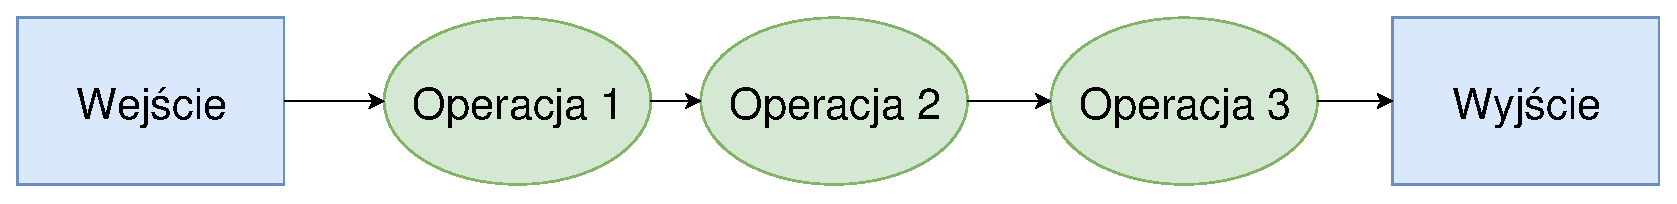
\includegraphics[width=1\textwidth]{img/batch}
	\caption{Procesowanie wsadowe}
  \label{fig:BatchProcessing}
\end{figure}
Takie podejście jest bardzo wygodne z punktu widzenia użytkowania,
po zdefiniowaniu wszystkich operacji oraz dostarczeniu danych wejściowych
proces nie wymaga żadnych dodatkowych czynności ze strony użytkownika.
Dodatkowo z uwagi na swój jednorazowy charakter wiadomo także czy operacje się udały czy nie.

Najpowszechniejszą architekturą wykorzystywaną w przetwarzaniu wsadowym jest \textit{Map Reduce}.
Schemat rozwiązania przedstawiono na rysunku \ref{fig:MapReduce}.
\begin{figure}[htbp]
\centering
	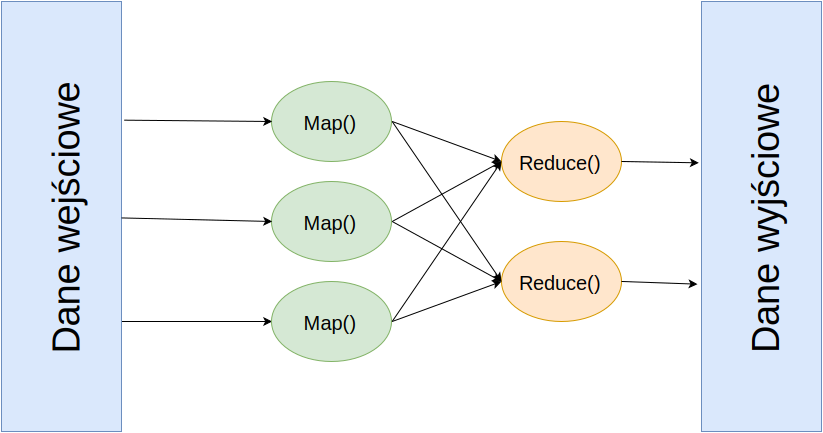
\includegraphics[width=0.9\textwidth]{img/mr}
	\caption{Model architektury rozwiązania \textit{Map Reduce}}
  \label{fig:MapReduce}
\end{figure}
Dane dzielone są na wiele,
niezależnych od siebie zbiorów,
na których wykonywane są różnego rodzaju przekształcenia,
operacje (faza \textbf{Map}).
Po wykonaniu wszystkich obliczeń następuje etap agregowania (faza \textbf{Reduce}) otrzymanych wyników.
Zyski z takiego podejścia najlepiej są widoczne w środowisku rozproszonym (wiele maszyn, procesów i wątków),
gdzie dzięki dekompozycji zadania wzrastają możliwości skalowania.

% TODO:
% Przykłady
% koszyk w supermarkecie

\subsection{Przetwarzanie strumieniowe}

Wymagania użytkowników co do czasu otrzymania wyniku
oraz pewna klasa problemów charakteryzujących się:
\begin{itemize}
	\item dużą szybkością napływania danych -- dane z czujników, sensorów, etc.,
	\item małymi opóźnieniami (\textit{latancy}) podczas przewarzania -- wykrywanie oszustw (\textit{fraud detection}),
\end{itemize}
powodują,
że metody przetwarzania wsadowego nie znajdują zastosowania.
Podejście strumieniowe polega na analizie danych bezpośrednio po ich pojawieniu się.
Nie jest istotny sposób w jaki dane się pojawiają,
ale fakt,
że są procesowane natychmiast po pojawieniu się.
Mechanizmy analizy strumieniowej można podzielić na 2 typy z uwagi na sposób przetwarzania:
\begin{itemize}
	\item \textbf{Niezależne}.
	Każdy nowy element (zdarzenie) jest przetwarzany pojedynczo i niezależnie od innych.
	Po wykonaniu operacji przekazywany jest do nowego strumienia bądź umieszczany w strumieniu wyjściowym.
	\item \textbf{Buforowane}.
	Elementy napływające ze strumienia przetrzymywane są przez zdefiniowany okres czasu
	bądź czekają na zebranie wystarczającej liczby elementów.
	Po spełnieniu wymaganego warunku są procesowane
	i tak jak w przypadku przetwarzania niezależnego przekazywane dalej albo na wyjście.
\end{itemize}

% TODO:
% Przykład

\section{Platformy streamingowe}
Ogromny potencjał drzemiący w analize danych w czasie rzeczywistym został dostrzeżony przez wiele firm.
Dlatego pierwsze rozwiązania powstawały wewnątrz departamentów \textit{IT},
dopiero potem będąc upublicznionym.
Dzięki temu na rynku dostępnych jest wiele rozwiązań oferujących analizę strumieniową.
Poprzez rozwiązania komercyjne od gigantów jak Microsoft, Google, Amazon,
po typu \textit{open-source},
takie jak Apache Storm, Apache Spark czy Apache Flink.

Wśród rozwiązań \textit{open-source} kilka cieszy się dość ugruntowaną pozycją na rynku,
przekładającą się na wiele udanych wdrożeń.
Są to:
\begin{itemize}
	\item Esper,
	\item Apache Spark,
	\item Apache Storm.
\end{itemize}


\section{Esper}
Esper jest silnikiem umożliwiającym złożoną analizę zdarzeń (ang. \textit{Complex Event Processing, CEP}).
Możliwość wbudowania w dowolną aplikację javy bądź .net.

Zalety:
\begin{itemize}
  \item język zbliżony do sql,
  \item prosta instalacja.
\end{itemize}

Wady:
brak wbudowanych mechanizmów zwiększających skalowalność.

\subsection{Apache Spark}
Spark jest narzędziem ogólnego przeznaczenia umożliwiającym przetwarzanie
i analizę dużych ilości danych.
Wykorzystywany jest z powodzeniem w operacjach związanych z:
\begin{itemize}
  \item uczeniem maszynowym,
  \item analizą skupień dużej ilości danych,
  \item analizą strumieniową.
\end{itemize}
Apache Spark charakteryzuje się:
\begin{itemize}
  \item \textbf{Łatwością w korzystaniu}.
  Dostarczony model programistyczny skrzętnie ukrywa szczegóły implementacyjne związane z procesowaniem rozproszonym.
  Dzięki temu programista może skupić się tylko na zadaniu.
  Dodatkowo dzięki wykorzystaniu popularnych języków (java, scala) próg wejścia jest relatywnie niski,
  a programy wykorzystywane przez Sparka są rozumiane nawet przez osoby nie zajmujące się przetwarzaniem danych.
  \item \textbf{Ogólnym przeznaczeniem}.
  Spark jest zintegrowaną platformą pozwalającą wykonywać wiele różnych zadań.
  Z powodzeniem można tworzyć zadania przetwarzania wsadowego,
  interaktywne analizy czy wykorzystywać mechanizmy uczenia maszynowego.
  \item \textbf{Skalowalnością}.
  Spark dostarcza mechanizmy umożliwiające skalowanie horyzontalne.
  Wystarczy dołączyć nową maszynę do klastra, aby poprawić osiągi systemu.
  Mechanizmy skalowania włączone są automatycznie,
  tzn. nie trzeba żadnych zmian w kodzie by mieć działający klaster.
  \item \textbf{Odpornością na awarie}.
  Spark sam automatycznie zarządza wszystkimi węzłami w klastrze
  i w razie awarii jest w stanie zareagować.
\end{itemize}

Oprócz standardowych mechanizmów Spark dostarcza zestaw dodatkowych funkcjonalności
w wydzielonych modułach (rys. \ref{fig:SparkModules}).
Są to operacje grafowe (GraphX), operacje SQL (Spark SQL), uczenie maszynowe (MLlib)
i przetwarzanie strumieniowe (Spark Streaming).
\begin{figure}[htbp]
  \centering
  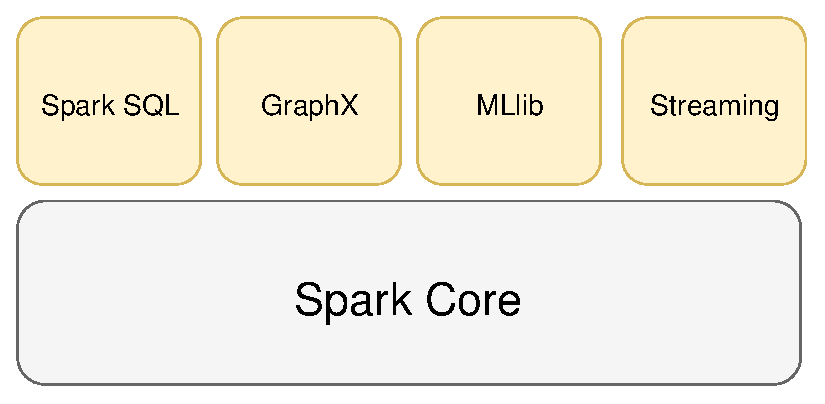
\includegraphics[width=0.7\textwidth]{img/sparkModules}
  \caption{Moduły Spark}
  \label{fig:SparkModules}
\end{figure}
\subsubsection*{Spark SQL}
Moduł dodający możliwość operowania na danych wykorzystywanych przez Sparka za pomocą języka SQL.
Pochodzenie danych nie ma znaczenia. Mogą być umieszone w
relacyjnych bazach danych, NoSQL, JSON, CSV czy innych ustrukturyzowanych formatach.
Szczegóły implementacyjne są skutecznie ukrywane.

Spark SQL można bezproblemowo wykorzystywać razem z innymi modułami (Spark Streaming, Spark ML czy GraphX).
Może być wykorzystywany zarówno w przetwarzaniu wsadowym historycznych danych
czy analizie strumieniowej w czasie rzeczywistym.
\subsubsection*{Spark GraphX}
Grapx dostarcza struktury danych umożliwiające na reprezentacje danych w formie grafów
zarówno sterowanych jak i niesterowanych.
Dodatkowo w tym module znajdują się przygotowana operatory i algorytmy umożliwiające prace z grafami.
\subsubsection*{Spark MLlib}
MLlib rozszerza Spark o dodatkowe funkcjonalności związane z uczeniem maszynowym (\textit{machine learning})
i analizą statystyczną.
Moduł ten zawiera wiele zaimplementowanych algorytmów między innymi do:
\begin{itemize}
  \item regresji liniowej (\textit{linear regression}),
  \item klasyfikatory Bayesa (\textit{Naive Bayes}),
  \item algorytmy do analizy skupień (\textit{cluster analysis}),
\end{itemize}
i wiele innych.
\subsubsection*{Spark Streaming}
Moduł Spark Streaming rozszerza podstawowe funkcjonalności o przetwarzanie strumieniowe danych.
Funkcjonalność przetwarzania strumieniowego zrealizowana jest poprzez mikro-buforowanie.
Strumień dzielony jest na mini-wsady o konfigurowalnym rozmiarze,
które dalej można przetwarzać za pomocą ogólnych (podstawowych) mechanizmów systemu Spark.

\subsection{Apache Storm}
Apache Storm jest framworkiem umożliwiającym strumieniowe przetwarzanie danych w czasie rzeczywistym.
Charakteryzuje się przy tym:
\begin{itemize}
  \item skalowalnością,
  \item odpornością na awarię,
  \item niezawodnością.
\end{itemize}
Stworzony został przez inżynierów z firmy
Backtype \footnote{\url{https://en.wikipedia.org/wiki/BackType}},
a po jej przejęciu, rozwijany przez inżynierów Twittera \footnote{\url{https://en.wikipedia.org/wiki/Twitter}}.
Obecnie projekt jest nadzworowany przez fundację Apache \footnote{\url{https://en.wikipedia.org/wiki/Apache_Software_Foundation}}.

Podobnie jak w przypadku Apache Storm zadanie jest odseparowane od wszelkich kwestii technicznych.

Centralnym punktem jest topologia (ang. \textit{topology}),
która reprezentuje zadanie w formie acyklicznego grafu skierowanego.
Graf ten ma 2 rodzaje węzłów.
\begin{itemize}
  \item \textit{Spouts} są źródłem danych w topologii.
  Pobierają je z zewnętrznego źródła i wprowadzają wewnątrz.
  \item \textit{Bolts} są miejscem,
  w którym następuje procesowanie danych: modyfikacja, filtracja czy agregacja.
\end{itemize}
Pomiędzy węzłami poruszają się krotki (ang. \textit{tuples}),
które są kontenerami na dane wyprodukawane przez węzły.
% budowa rysunek
\begin{figure}[htbp]
\centering
	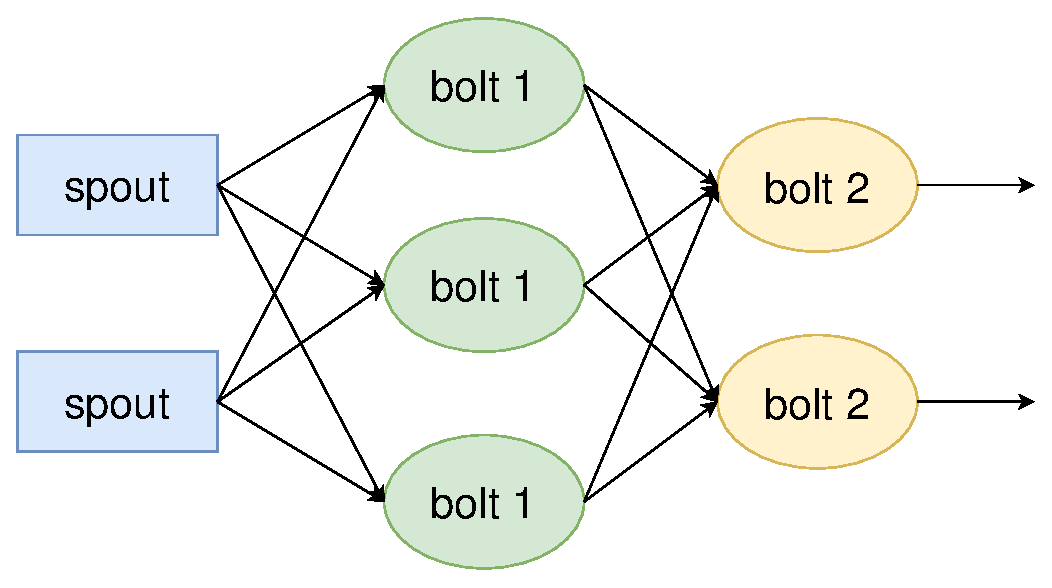
\includegraphics[width=1\textwidth]{img/storm}
	\caption{Topologia rozwiązania Apache Storm}
  \label{fig:StormTopology}
\end{figure}
% at least once
należy być przygotowanym,
że wiadomość może zostać przetworzona więcej niż jeden raz


\section{Podsumowanie}

Wszystkie opisane frameworki służą do obsługi przetwarzania strumieniowego.
Mimo że służą do podobnych zastosowań,
pomiędzy nimi istnieją zasadnicze różnice.
Zarówno w obsłudze danych,
jak i w podejściu do samego przetwarzania.

W ramach niniejszej pracy wcześniej wymienione platformy zostały sprawdzone pod kątem:
\begin{itemize}
  \item możliwości jakie oferują,
  \item sposobu korzystania zarówno od strony użytkownika jak i programisty.
\end{itemize}

\subsubsection*{Sposób procesowania, opóźnienia, skalowalność}
Największą różnicą pomiędzy omawianymi platformami jest tryb w jakim procesowane są zdarzenia.
Spark buforuje (zbiera) napływające dane w zadanym interwale czasu i dopiero potem procesuje,
natomiast procesuje dane bezpośrednio po ich otrzymaniu.
Esper dzięki swoim wbudowanym mechanizmom może pracować w obydwu trybach.

Różne tryby przetwarzania mają swoje konsekwencje w opóźnieniach (\textit{latency}).
Spark z uwagi na występowanie okien czasowych ma je zauważalne,
z kolei Storm przetwarzający dane od razu ma opóźnienia praktycznie pomijalnie małe.

Sposób przetwarzania ma także wpływ na gwarancje jakie oferują frameworki.
Ponieważ Spark nie musi pilnować pojedynczo danych,
tylko mini-batche może zagwarantować,
że dane zdarzenie przeprocesuje się dokładnie raz (\textit{exacly once}).
Storm natomiast śledzi wszystkie rekordy indywidualnie jak poruszają się przez system,
dlatego jedyne gwarancje jakie daje,
to że dane zostaną przeprocesowane co najmniej raz (\textit{at least once}).
Powoduje to, że mogą pojawić się duplikaty - niektóre rekordy mogą być przeprocesowane więcej niż jeden raz,
na przykład podczas awarii węzła.
Esper natomiast jest tylko silnikiem osadzanym wewnątrz innych aplikacji,
nie ma wbudowanych mechanizmów zarządzania klastrami,
dlatego problem zachowania gwarancji nie istnieje.
\begin{table}[h]
  \label{tab:ModelComparison}
  \begin{tabular}{p{0.2\linewidth} | p{0.25\linewidth} | p{0.25\linewidth} | p{0.2\linewidth}}
    & Esper & Spark & Storm \\
    \hline
    typ & silnik CEP & ogólny & ogólny \\
    \hline
    model & obydwa & buforowanie & niezależne \\
    \hline
    gwarancje & co najwyżej raz & co najwyżej raz & co najmniej raz \\
    \hline
    skalowalność & nie & tak & tak \\
  \end{tabular}
  \caption{Porównanie platform}
\end{table}

\subsubsection*{Implementacja, API programistyczne}
Storm w większości został napisany w języku Clojure.
API programistyczne jest przygotowane dla javy,
jednak można wykorzystywać je we wszystkich językach wykorzystujących wirtualną maszynę (\textit{jvm}).
Dodatkowo elementy Storma może wykonywać skrypty napisane w innych językach: python, R, etc.
Spark został napisany w scali,
posiada przygotowane API w javie, scali i R.
Esper powstał w języku java, chociaż posiada port napisany w języku C\#.
Do wykonywania operacji na danych wykorzystuje własny język oparty na SQL.
\begin{table}[h]
  \label{tab:ProgrammingApi}
  \begin{tabular}{p{0.2\linewidth} | p{0.25\linewidth} | p{0.25\linewidth} | p{0.2\linewidth}}
    & Esper & Spark & Storm \\
    \hline
    napisany w & java & scala & clojure \\
    \hline
    api & java, C\# & jvm, python, R & wiele \\
  \end{tabular}
  \caption{Porównanie platform -- API}
\end{table}

\subsubsection*{Instalacja, użytkowanie}
Najprostszym sposobem instalacji cechuje się Esper.
Biblioteka ma formę pojedynczego pliku, który łatwo podpiąć pod istniejące aplikacje.
System storm posiada dwa tryby lokalny i zdalny.
Tryb lokalny pozwala na tworzenie topologii na komputerach bez konieczności tworzenia klastrów.
Dzięki temu programiści mają ułatwione możliwości rozwoju aplikacji czy szukania przyczyn błędów.
Tryb zdalny jest przeznaczony dla klastrów.
Topologie w formie archiwum przesyła się do nadzorcy klastra,
a on już rozpropagowuje ją wewnątrz.
Apache Spark jest niestety pozbawiano trybu lokalnego.
Trzeba stworzyć klaster składający się z jednego węzła.

Esper charakteryzuje się także najprostszym sposobem operowania na strumieniach.
Dostarczony własny język jest bardzo ekspresywny i bogaty w funkcjonalności.
W przypadku Apache Spark dostęp do danych jest ukryty za pomocą wewnętrznych struktur.
Dzięki takiemu podejściu na start dostępnych jest wiele funkcjonalności,
jednak próba utworzenia dodatkowych elementów nie zawsze może skończyć się sukcesem.
Brak trybu lokalnego nie ułatwia tworzenia testowych źródeł danych.
Apache Storm jest najbardziej generycznym narzędziem.
Większość elementów trzeba wykonać samodzielnie,
przez co próg wejścia jest większy niż w przypadku pozostałych frameworków.
\begin{table}[h]
  \label{tab:ProgrammingLevel}
  \begin{tabular}{p{0.2\linewidth} | p{0.25\linewidth} | p{0.25\linewidth} | p{0.2\linewidth}}
    & Esper & Spark & Storm \\
    \hline
    instalacja & pojedynczy jar & cały projekt & tryb lokalny/zdalny \\
    \hline
    użytkowanie & własny DSL & wewnętrzne api & wewnętrzne api i dowolne skrypty
  \end{tabular}
  \caption{Porównanie platform -- instalacja}
\end{table}


\chapter{Analiza sytuacji nietypowych}
\label{chap:ChangeDetectionAlgo}
\section{Wprowadzenie}

Sytuacje nietypowe są to takie sytuacje,
które odbiegają od normalnie obserwowanych zachowań.
Może to być awaria, przeciążenie systemów,
trwający atak komputerowy z zewnątrz czy próba oszustwa.

Wykrywanie zmian (\textit{changepoint detection}) jest procesem
wykrycia w strumieniu czasowym wzorców (zmian zachowań, charakterystyk) nie pasujących do wcześniej zaobserwowanych.
Zmiany mogą mieć wiele różnych form.
Strumień danych może w pewnym momencie charakteryzować się rozkładem Gaussa,
aby nagle zmienić się na rozkład Poissona.
Przykładem takiej formy jest zachowanie czujnika światła (rys. \ref{fig:SignalDevice}).
W ciągu dnia, gdy jest słoneczna pogoda na chwilowe wartości może mieć wpływ zachmurzenie, przechodzące osoby, itp.
W nocy wahania są mniejsze.
\begin{figure}[htbp]
\centering
	\includegraphics[width=0.6\textwidth]{img/ch-2-device}
	\caption{Wartości czujnika światła -- wahania w rytmie dzień/noc}
  \label{fig:SignalDevice}
\end{figure}
Inną formą może być zmiana parametrów rozkładu.
Przykładowo w strumieniu opisanym rozkładem Gaussa
w pewnym momencie czasu mogło nastąpić przesunięcie średniej (rys. \ref{fig:SignalData}).
\begin{figure}[htbp]
\centering
	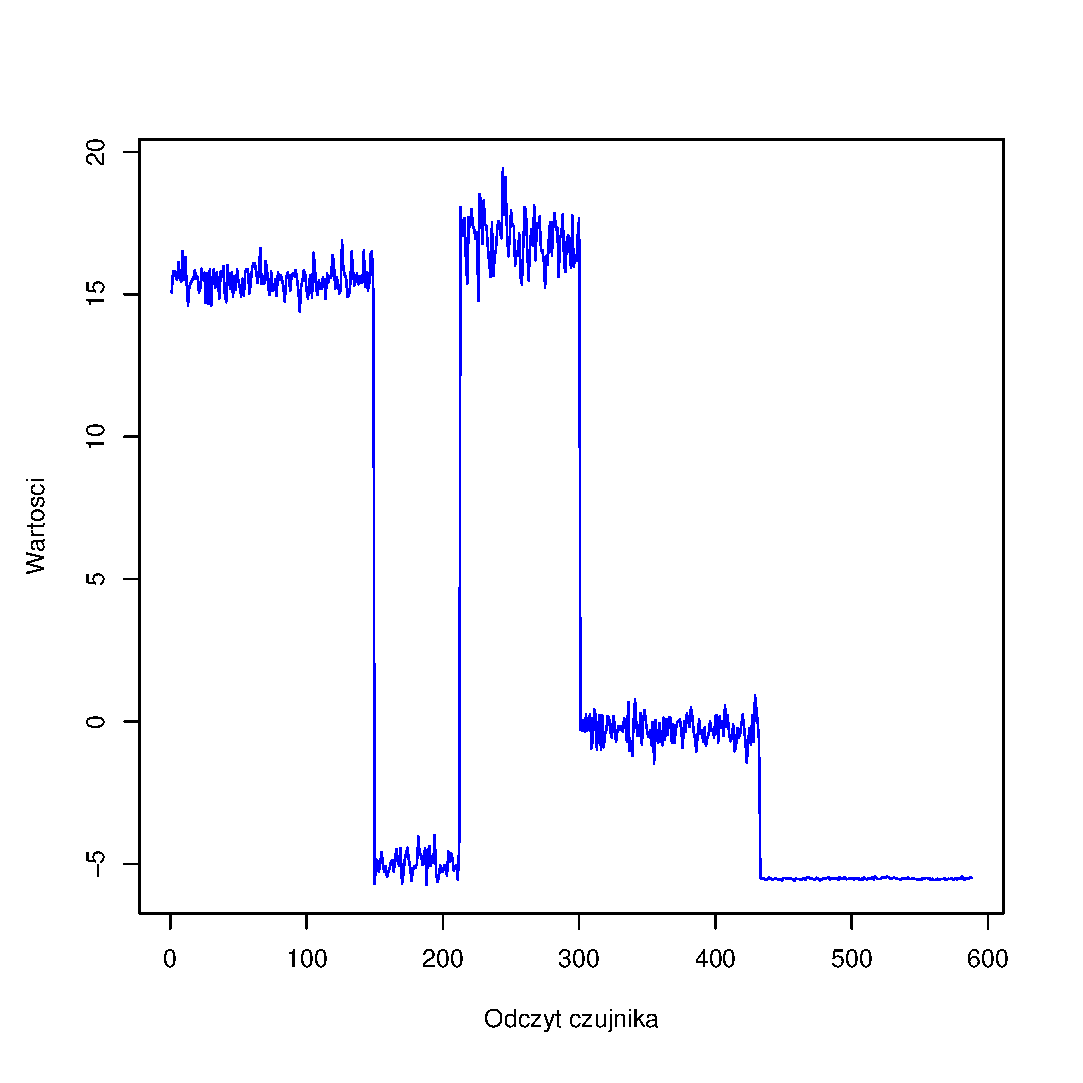
\includegraphics[width=0.6\textwidth]{img/ch-2-data}
	\caption{Zmiana parametrów opisujących strumień danych}
  \label{fig:SignalData}
\end{figure}

% \begin{figure}[htbp]
% \centering
% 	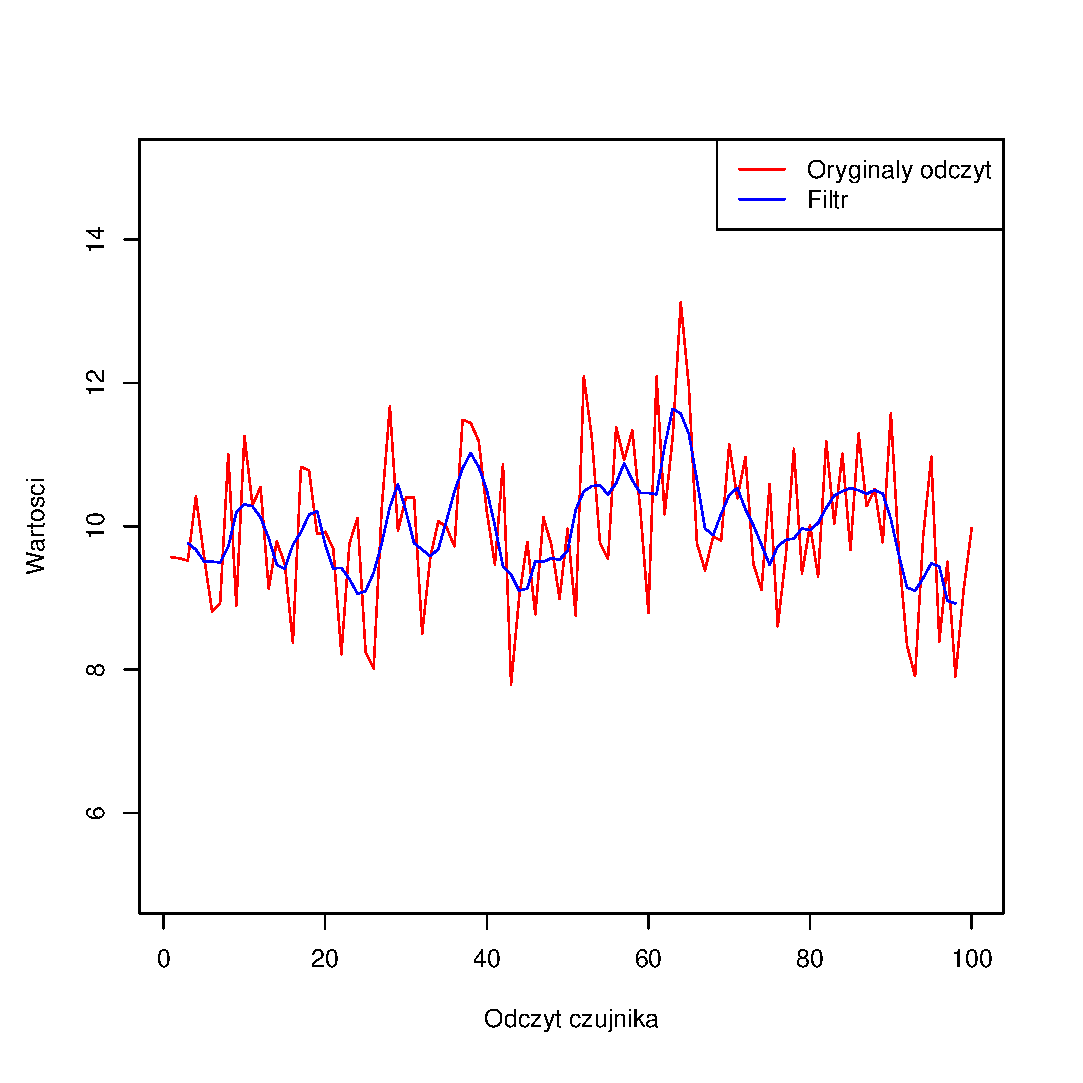
\includegraphics[width=0.5\textwidth]{img/ch-2-filter}
% 	\caption{Procesowanie wsadowe}
%   \label{fig:SignalFilter}
% \end{figure}

\section{Metody wykrywania zmian}

Przez lata z uwagi na swoje znaczenie problem wykrywania zmian skupiał uwagę naukowców i badaczy.
Powstało wiele metod starających się go rozwiązać.
Większość z nich opiera się na:
\begin{itemize}
  \item wartościach progowych,
  \item metodach analitycznych,
  \item analizie skupień (\textit{cluster analysis}),
  \item elementach uczenia maszynowego.
\end{itemize}
W dalszej częsci rozdziału zostaną omówione wartości progowe i metody analityczne
\subsection{Wartości progowe}
Najprostszym sposobem wykrywania sytuacji nietypowych jest ustalenie wartości progowej (\textit{threshold value}),
której przekroczenie oznacza wystąpienie zmiany.
Przykład przedstawiono na rysunku \ref{fig:SignalThreshold}.
Podejście jednak taki wiąże się z pewnymi ograniczeniami.
Dane muszą się charakteryzować względną stabilnością,
tj. powinny mniej więcej utrzymywać się na tym samym poziomie, wzrastać tylko podczas sytuacji nietypowych.
Charakterystyka danych,
także musi być znana,
aby można było dobrać odpowiednią wartość progu.
Strategia skutecznie stosowana w:
\begin{itemize}
  \item systemach awaryjnych,
  \item systamach monitorujących.
\end{itemize}
\begin{figure}[htbp]
\centering
	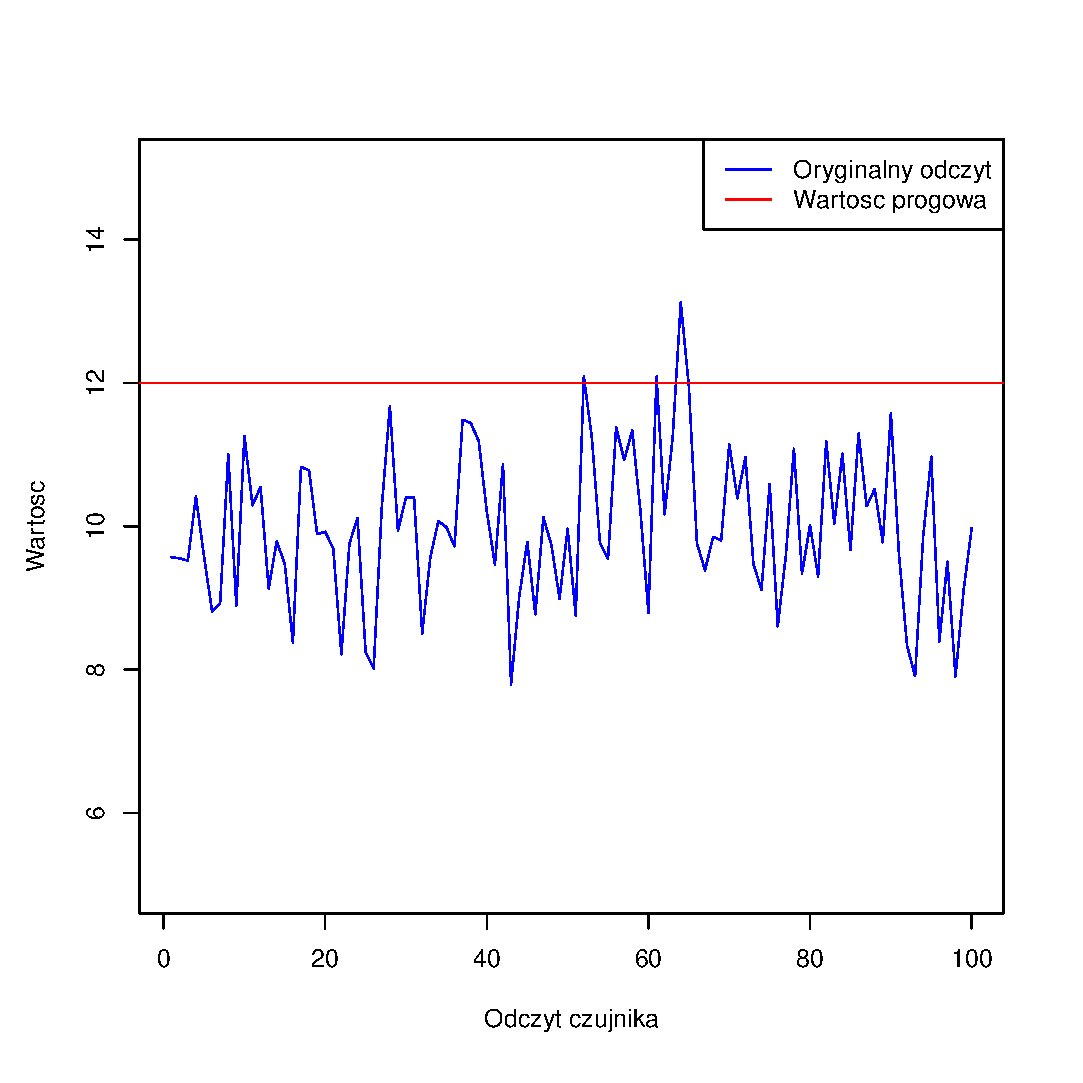
\includegraphics[width=0.6\textwidth]{img/ch-2-threshold}
	\caption{Wykrywanie sytuacji nietypowych -- wartość progowa}
  \label{fig:SignalThreshold}
\end{figure}

\newpage
\subsection{Metody analityczne}

Metody analityczne do rozwiązania problemu wykrywania zmian wykorzystują aparat matematyczny,
głównie statystykę.
Budują na podstawie otrzymywanych danych
oraz wewnętrznego modelu funkcję prawdopodobieństwa wystąpienia sytuacji nietypowej.
Na jej podstawie możliwe jest wtedy podjęcie decyzji.
Na rysunku \ref{fig:SignalAnalytics} przedstawiono strumień,
w którym wystąpił szereg zmian.
Poniżej znajduję się odpowiadająca funkcja opisująca prawdopodobieństwo wystąpienia zmiany w tym strumieniu.
\begin{figure}[htbp]
\centering
	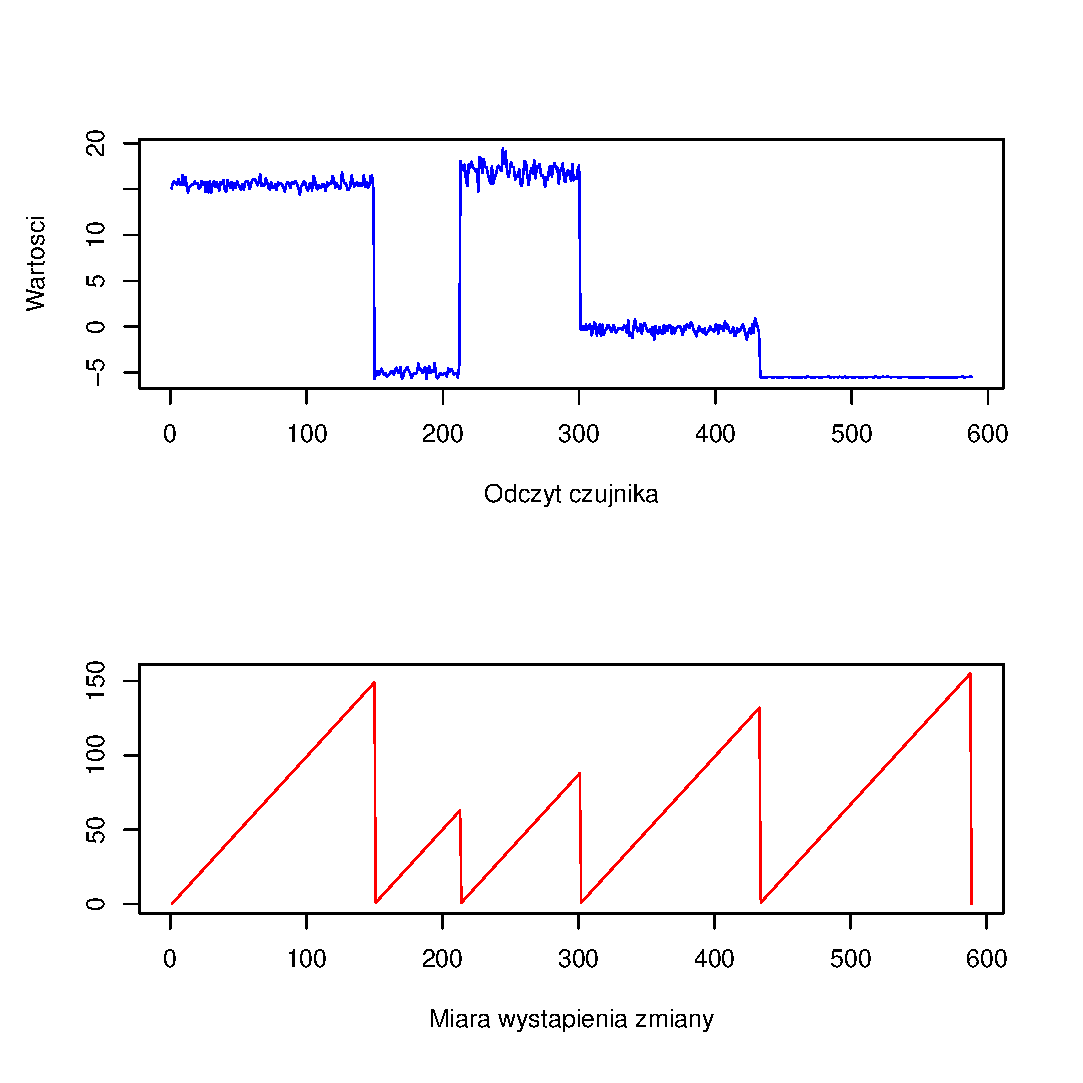
\includegraphics[width=1\textwidth]{img/ch-2-change}
	\caption{Wykrywanie sytuacji nietypowych -- funkcja prawdopodobieństwa}
  \label{fig:SignalAnalytics}
\end{figure}

Metody analityczne dzielą się na dwie grupy:
\begin{itemize}
  \item \textbf{offline} -- wymagają całego zestawu danych,
  \item \textbf{online} -- przyrostowo analizują dane.
\end{itemize}
Metody offline charakteryzują się większą dokładnością wyników,
za cenę większych opóźnień.
Są wykorzystywane w analizach danych z czujników pogodowych, segmentacji DNA, itp.
Metody online mają praktycznie niezauważalne opóźnienia,
obarczone są jednak większymi błędami.


\chapter{Algorytmy wykrywania zmian}
\section{Algorytm Bayesa}
\label{sec:Bayes}

\section{ADWIN}
\label{sec:ADWIN}
ADWIN należy do grupy algorytmów opartych na koncepcji przesuwnego okna (\textit{sliding window}).
Okno jest zbiorem badanych rekordów o najczęściej jawnie wcześniej zdefiniowanym rozmiarze (rys. \ref{fig:SlidingWindowInit})
do którego wkładane są najnowsze próbki, starsze natomiast są usuwane (rys. \ref{fig:SlidingWindowMove}).
\begin{figure}[htbp]
\centering
	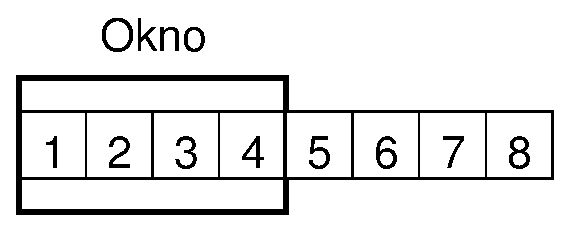
\includegraphics[width=0.5\textwidth]{img/slidingWindowInit}
	\caption{Przesuwne okno - początek}
  \label{fig:SlidingWindowInit}
\end{figure}
\begin{figure}[htbp]
\centering
	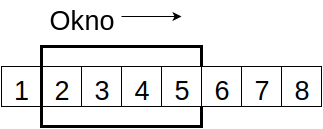
\includegraphics[width=0.5\textwidth]{img/slidingWindowMove}
	\caption{Przesuwne okno - przesuwanie}
  \label{fig:SlidingWindowMove}
\end{figure}
Na podstawie zawartości okna algorytmy mogą:
\begin{itemize}
  \item sprawdzić czy nie zaszła zmiana,
  \item przebudować, zaktualizować model.
\end{itemize}
Dlatego wielkość okna ma znaczenie.
Im jest dłuższe tym algorytmy zachowują się stabilniej w spokojnych okresach,
natomiast im krótsze tym szybciej reagują na zmiany.

Algorytm ADWIN (\textit{ADaptive WINdow}) zaproponowany przez Bifeta (Bifet i in., 2011)
wykorzystuje okno, jednak jego rozmiar jest dynamiczny,
tj. nie ma ustalonego wymiaru i zmienia się w czasie, w zależności od procesowanych danych.

Głównym elementem algorytmu jest przesuwne okno $W$,
którego zawartością są aktualne rekordy $x_{i}$.
W raz z pojawieniem się nowych próbek wewnątrz okna
sprawdzane jest czy wszystkie dostatecznie duże pod-okna nie różnią się względem siebie za bardzo.
Jeśli są różniące się pod-okna to znaczy,
że nastąpiła zmiana. Na koniec kasowane jest starsze pod-okno.
Minimalna wielkość pod-okna i sposób ich porównania zależą od wybranego testu statystycznego
na zgodność rozkładów pod-okien.
\subsection{Testy rozkładu -- średnia, wariancja}
\label{sub:TestsMeanAndVar}
Najprostszym sposobem na sprawdzenie czy dwa pod-okna nie różnią się od siebie
jest sprawdzenie czy ich średnie nie różnią się od siebie.
Można to zapisać
$$ | \hat{\mu}_{W_{0}} - \hat{\mu}_{W_{1}} | < \varepsilon, $$
gdzie $W_{0}$ i $W_{1}$ to pod-okna, a $\varepsilon$ to wartość progowa.

Gdy $n_{0}$ to rozmiar $W_{0}$,
a $n_{1}$ to rozmiar $W_{1}$ cały test można zapisać (Bifet i in., 2011)
$$n = n_{0} + n_{1}$$
$$q^\prime = \frac{q}{n}$$
$$m=\frac{1}{\frac{1}{n_0}+\frac{1}{n_1}}$$
$$\varepsilon = \sqrt{\frac{2}{m} \sigma^{2}_{W} \mbox{ln}\frac{2}{q^\prime}} + \frac{2}{3m} + \mbox{ln}\frac{2}{q^\prime},$$
gdzie $\sigma^{2}_{W}$ to wariancja całego okna $W$,
a $q$ to poziom istotności testu.
\subsection{Testy rozkładu -- stosunek gęstości}
\label{sub:TestDensityRatio}
Przedstawiony wcześniej test sprawdza się dobrze,
gdy dane można opisać rozkładem normalnym.
Gdy jednak dane pochodzą z innych rozkładów albo mają więcej wymiarów pojawiają się problemy.
Tych mankamentów nie ma test opisany poniżej.

Dane $x_1,x_2,\ldots,x_t,\ldots \in \mathbb{R}^n$ i mogą pochodzić z różnych rozkładów.
Niech
$$ Y(t) = [{x_t, x_{t+1}, x_{t+2}, \ldots, x_{t+n-1}}]$$
będzie podzbiorem próbek zaczynającym się w chwili $t$.
Zmianą można nazwać,
gdy dla dwóch następujących po sobie zbiorów $Y(t)$ i $Y(t+n)$
wartość miary opisującej ich róznice jest wystarczająco duża.

Do popularnych miar rozbieżności opartych na rozkładach prawdopodobieństaw należy miara Kullbacka-Leiblera:
$$\mbox{KL}(P||P^\prime) = \int p(\textbf{Y}) \mbox{log}\frac{p(\textbf{Y})}{p^\prime(\textbf{Y})} \mbox{d}\textbf{Y},$$
gdzie $P$ to rozkład prawdopodobieństwa zbioru $Y(t)$,
$P^\prime$ zbioru $Y(t+n)$,
natomiast $p(\textbf{Y})$ i $p^\prime(\textbf{Y})$ to funkcje gęstości rozkładów $P$ i $P^\prime$.

Początkowo badacze starali się obliczyć $p(\textbf{Y})$ i $p^\prime(\textbf{Y})$ osobno
i dopiero potem wyliczyć ich stosunek.
Jednak takie podejście okazało się trudne.
Sugiyama (Sugiyama i in., 2008) w swojej pracy zaproponował próbę bezpośredniego przybliżenia stosunku gęstości.
$$\hat{\mbox{KL}} = \frac{1}{n} \sum\limits_{i=1}^n \mbox{log}\,\hat{g}(\textbf{Y}_i),$$
gdzie $\hat{g}(\textbf{Y}_i)$ jest estymatorem stosunku gęstości.

Wartość estymatora otrzymujemy
$$\hat{g}(\textbf{Y}) = \sum\limits_{l=1}^n \hat{\theta}_l K(\textbf{Y}, \textbf{Y}_l)$$


\chapter{Badania eksperymentalne}
\section{Organizacja eksperymentów}
W poniższym rozdziale wybrane modele z rozdziału \ref{chap:ChangeDetectionAlgo} zostaną,
w celu zbadania efektywności algorytmów,
przetestowane na losowych zbiorach danych.
Sekcja ta została podzielona na dwie części.
Pierwsza przedstawia szczegółową analizę problemu z wykorzystaniem badanych metod,
natomiast w części drugiej znajdują się zbiorcze wyniki przeprowadzonych doświadczeń.

Analizie eksperymentalnej zostaną poddane algorytmy:
\begin{itemize}
  \item Bayesa,
  \item ADWIN z testem opartym o średnią,
  \item ADWIN z testem opartym o stosunek gęstości rozkładu.
\end{itemize}

W badaniach będą wykorzystane zbiory danych wygenerowane losowo jak i rzeczywiste,
pochodzące z prawdziwych czujników.
\subsection*{Dane wygenerowane losowo}
\subsubsection*{Skacząca średnia}
Jednowymiarowy model auto-regresji wykorzystany przez Liu (Liu i in., 2013)
zostanie użyty do wygenerowania 5000 próbek.
Wartości są opisane wzorem:
$$y(t) = 0.6y(t-1) - 0.5y(t-2) + \varepsilon_t,$$
gdzie $\varepsilon_t$ jest szumem opisanych rozkładem Gaussa z średnią $\mu$
i odchyleniem standardowym równym 1,5.
Zmianie co 100 próbek ulegała średnia szumu $\mu$.
\[ \mu_N =
  \begin{cases}
    0       & \quad N = 1\\
    \mu_{N-1} + \frac{N}{16} & \quad N = 2,3, \ldots, \\
  \end{cases}
\]
gdzie N to liczba naturalna równa indeksowi aktualnej zmiany.
\subsubsection*{Rozkład dwuwymiarowy -- zamiana kowariancji}
Do badania użyto 5000 próbek pobranych z dwuwymiarowego rozkładu normalnego.
Zmiana występuje co 100 próbek
i polega na modyfikacji macierzy kowariancji $\Sigma$.
\[ \Sigma =
  \begin{cases}
    \begin{pmatrix} 1 & -\frac{4}{5} - \frac{N-2}{500} \\ -\frac{4}{5} - \frac{N-2}{500} & 1 \end{pmatrix} & \quad N = 1,3,\ldots\\
    \begin{pmatrix} 1 & \frac{4}{5} + \frac{N-2}{500} \\ \frac{4}{5} + \frac{N-2}{500} & 1 \end{pmatrix} & \quad N = 2,4,\ldots\\
  \end{cases}
\]
\subsubsection*{Badanie sprawności}
Do oceny sprawności algorytmów wykorzystano miary zapraponowane przez Liu (Liu i in., 2013):
\begin{itemize}
  \item współczynnik sukcesów (\textit{true positive rate, TPR}): $n_{s}/n_{c}$,
  \item wspólczynnik fałszywych alarmów (\textit{false positive rate, NPR}): $(n_{a}-n_{s})/n_{a}$,
\end{itemize}
gdzie $n_{s}$ to liczba poprawnie wykrytych zmian, $n_{c}$ to liczba wprowadzonych zmian,
a $n_{a}$ to liczba wszystkich wykrytych zmian.

\subsection*{Dane rzeczywiste}
Dane rzeczywiste zebrano za pomocą czujnika światła oraz czujnika zbiżeniowego.
Czujniki leżały na biurku i skierowane pionowo w kierunku sufitu.
Przykładowe wyniki czujników przedstawiono w tabeli \ref{tab:DeviceValues}.
Wykres \ref{fig:DeviceValues} przedstawia przebiegi ostatnich 5000 próbek.
\subsubsection*{Czujnik światła}
Czujnik mierzył natężenie światła w otoczeniu.
Na wartości wpływ ma nie tylko fakt przesłonięcia go przez przedmiot,
ale także pora dnia.
\subsubsection*{Czujnik odległości}
Czujnik zbliżeniowy mierzy odległość od najbliższego przedmiotu,
wynik był podawany w cm.
\begin{table}[h]
  \label{tab:DeviceValues}
  \centering
  \begin{tabular}{r r}
    \multicolumn{1}{l}{Odległość} & \multicolumn{1}{l}{Natężenie} \\
    \hline
    266.34 & 0566 \\
    266.34 & 0567 \\
    266.32 & 0566 \\
    266.77 & 0566 \\
    266.84 & 0567 \\
    266.36 & 0567 \\
    266.73 & 0568 \\
    266.29 & 0566 \\
    266.68 & 0565 \\
    266.29 & 0566 \\
    266.36 & 0566 \\
    266.32 & 0567 \\
    266.72 & 0568 \\
    266.77 & 0567 \\
  \end{tabular}
  \caption{Wartości czujników}
\end{table}
\begin{figure}[htbp]
  \centering
  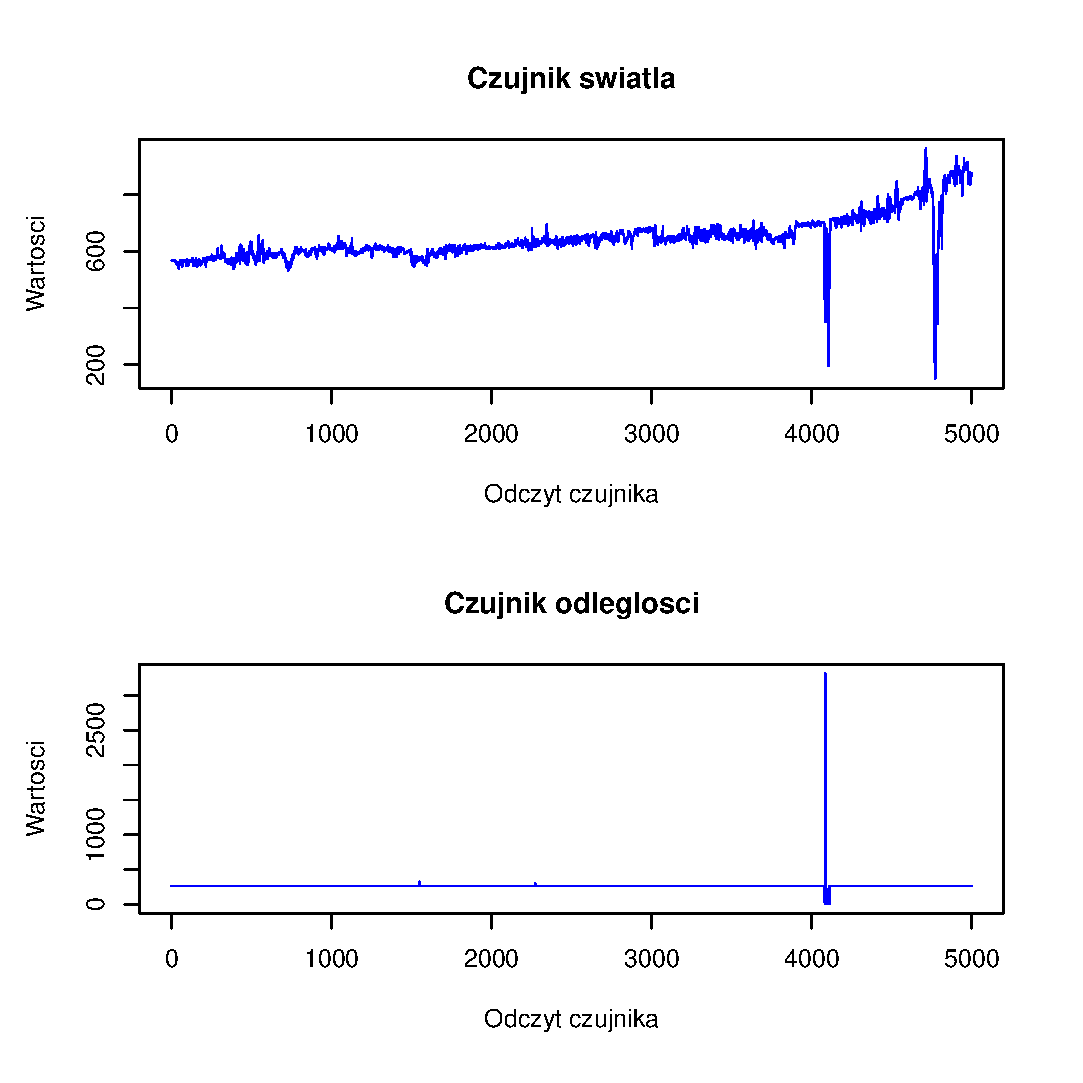
\includegraphics[width=1\textwidth]{img/ch-5-device}
  \caption{Wartości czujników}
  \label{fig:DeviceValues}
\end{figure}
\newpage
\section{Wyniki eksperymentów}
W poniższym rozdziale zostaną przedstawione wyniki przeprowadzonych badań.
\subsection{Skacząca średnia}
Na wykresie \ref{fig:JumpingValues} przedstawiono przykładowy przebieg wartości dla pierwszych 5 zmian
wraz z zaznaczonymi miejscami,
gdzie nastąpiła.
\begin{figure}[htbp]
  \centering
  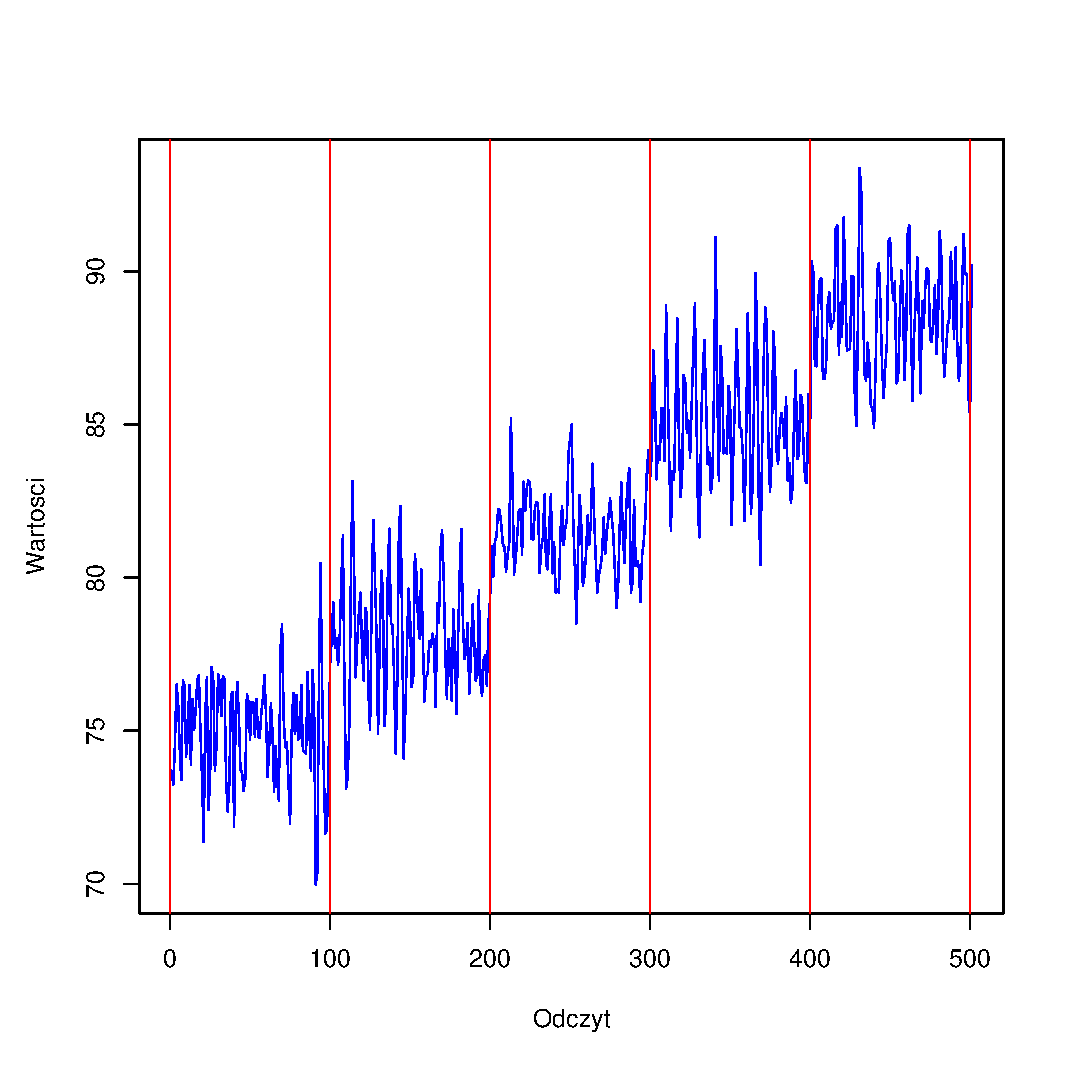
\includegraphics[width=0.8\textwidth]{img/ch-5-jumping}
  \caption{Przykładowe wartości}
  \label{fig:JumpingValues}
\end{figure}
Badanie przeprowadzono poprzez wygenerowanie 20 zestawów danych.
Źródło (\textit{seed}) dla każdego z zestawów były inne.
Dla wszystkich zestawów w tabeli \ref{tab:JumpingResult} przedstawiono średnią oraz wariancje współczynników sukcesu i fałszywych alarmów.
\begin{table}[h]
  \label{tab:JumpingResult}
  \centering
  \begin{tabular}{l r r r r}
    & \multicolumn{2}{l}{TPR} & \multicolumn{2}{l}{NPR} \\
    \hline
    & \multicolumn{1}{l}{Średnia} & \multicolumn{1}{l}{Wariancja}& \multicolumn{1}{l}{Średnia} & \multicolumn{1}{l}{Wariancja} \\
    \hline
    BAY & 0,439 & $0,887 \times 10^{-3}$ & 0,689 & $1,213 \times 10^{-3}$  \\
    $ADW_{\mu}$ & 0,526 & $1,246 \times 10^{-3}$ & 0,727 & $1,539 \times 10^{-3}$ \\
    $ADW_{d}$ & 0,516 & $2,508 \times 10^{-3}$ & 0,712 & $2,627 \times 10^{-3}$ \\
  \end{tabular}
\end{table}

\begin{figure}[htbp]
  \centering
  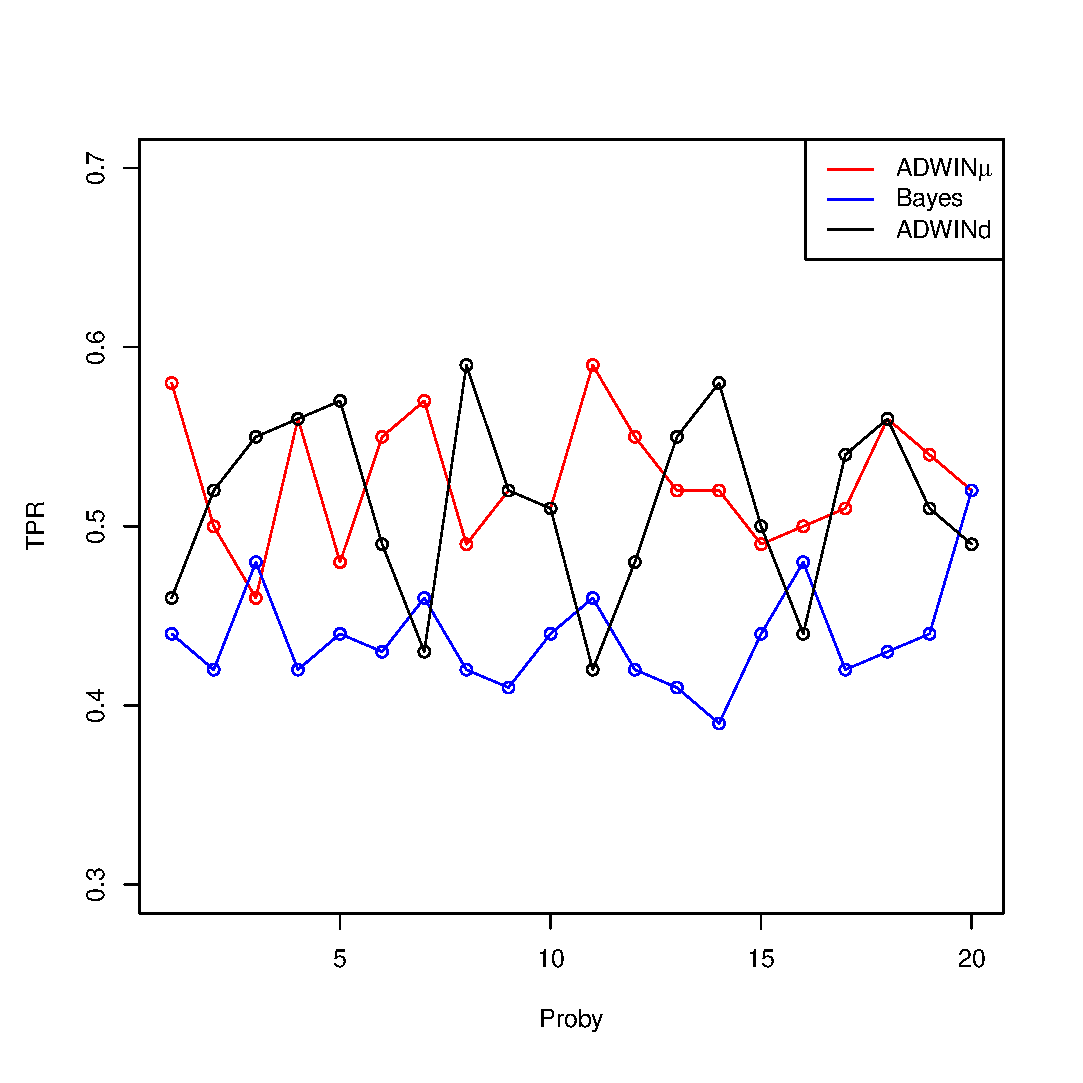
\includegraphics[width=0.5\textwidth]{img/ch-5-jump-res-tpr}
  \caption{Wyniki dla poszczególnych prób -- współczynnik suksesów}
  \label{fig:JumpingValuesResTpr}
\end{figure}
\begin{figure}[htbp]
  \centering
  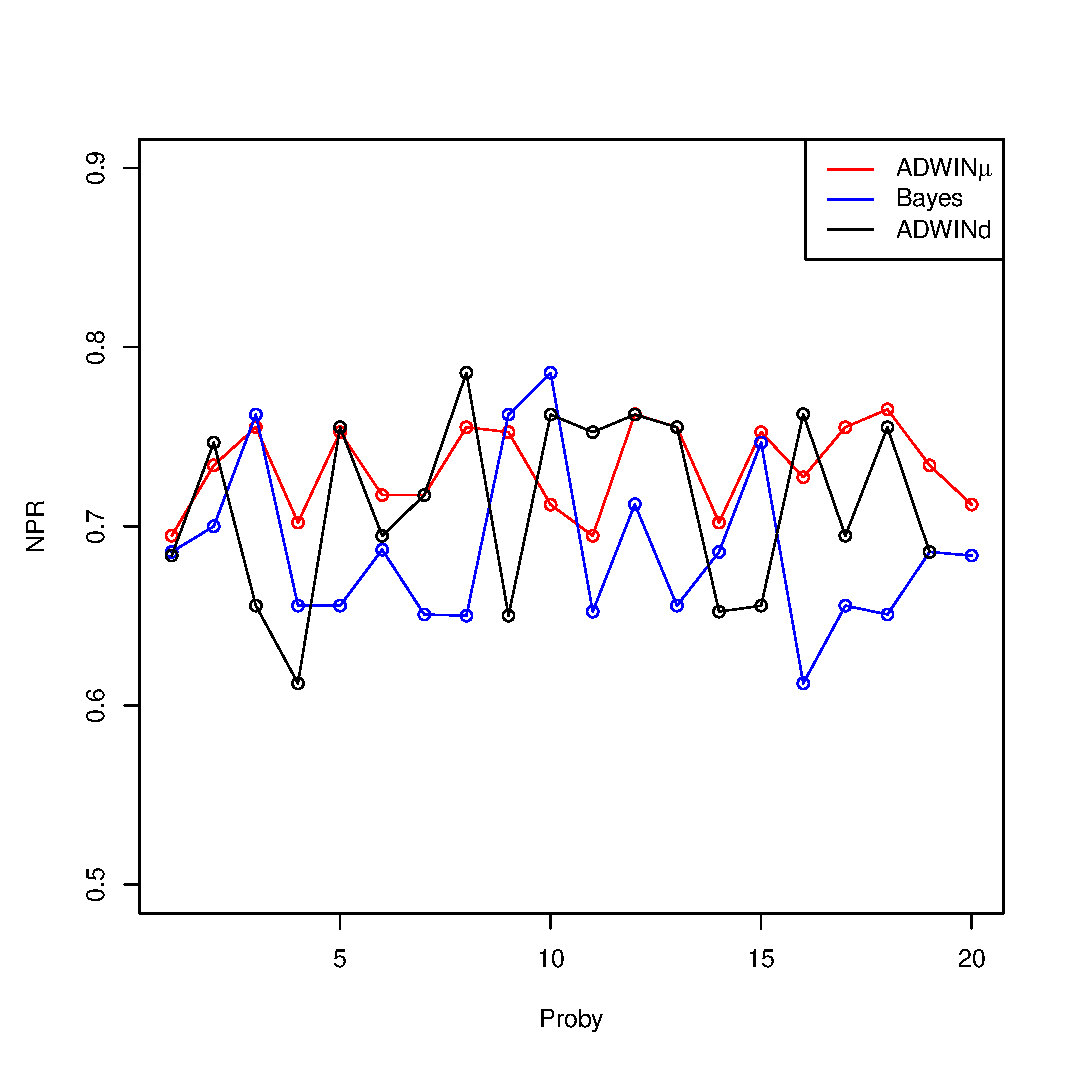
\includegraphics[width=0.5\textwidth]{img/ch-5-jump-res-npr}
  \caption{Wyniki dla poszczególnych prób -- współczynnik fałszywych alarmów}
  \label{fig:JumpingValuesResTpr}
\end{figure}

\subsubsection{Zamiana kowariancji}
Na wykresie \ref{fig:CovValues} przedstawiono przykładowy przebieg wartości dla pierwszych 5 zmian
wraz z zaznaczonymi miejscami,
gdzie nastąpiła.
\begin{figure}[htbp]
  \centering
  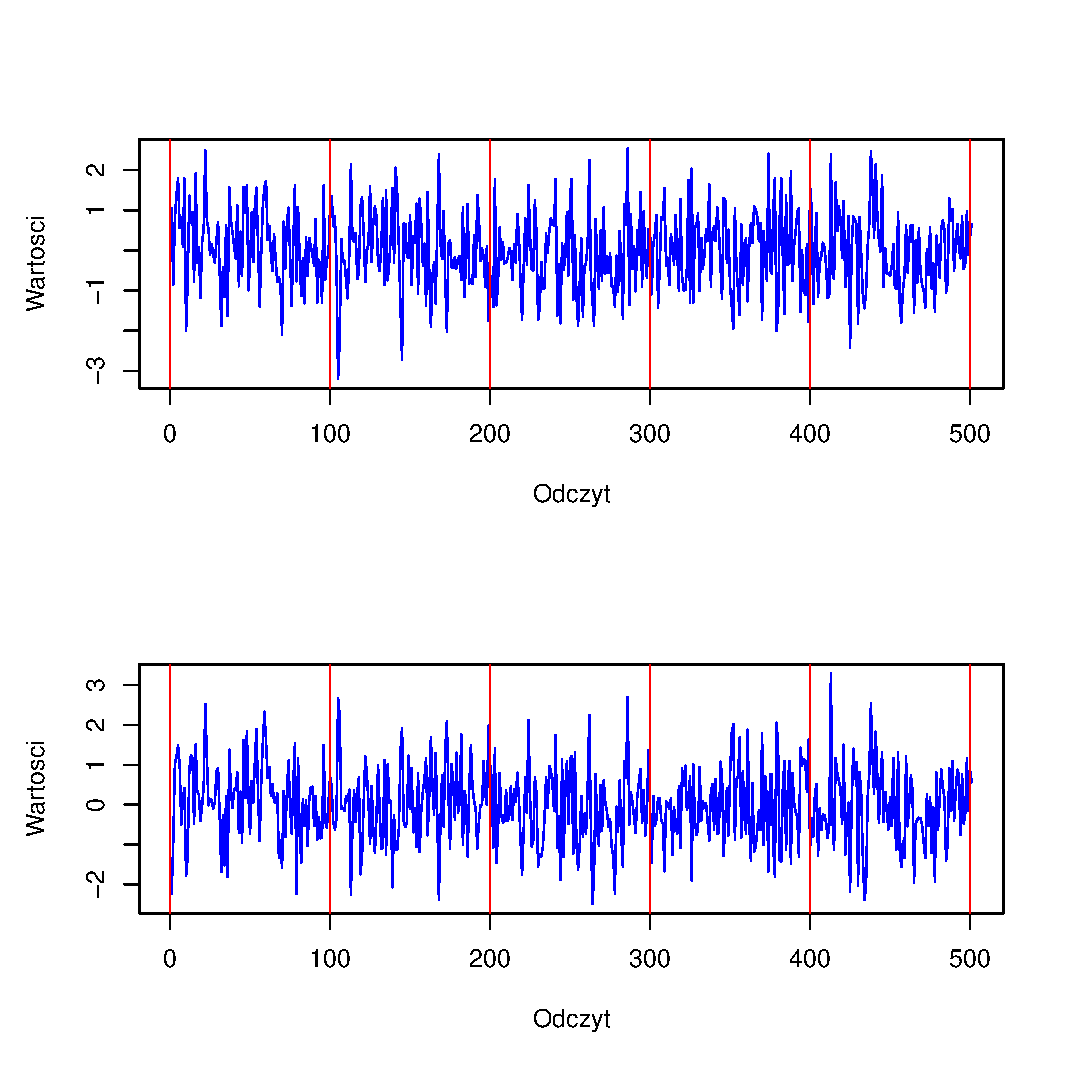
\includegraphics[width=0.8\textwidth]{img/ch-5-cov}
  \caption{Przykładowe wartości}
  \label{fig:CovValues}
\end{figure}
Na górnym rysunku przedstawiono pierwszy wymiar, na niższym drugi.
Badanie przeprowadzono poprzez wygenerowanie 20 zestawów danych.


\chapter{Zakończenie}
W ramach pracy magisterskiej została przedstawione zagadnienie wykrywania zmian w kontekscie analizy strumieniowej.
Dokonano przeglądowej analizy jakościowej i wydajnościowej wybranych platform z rozdziału \ref{ch:tech}.
Z wykorzytniem Apache Storm zostały zaimplementowane algorytmy z rodziału \ref{ch:algo},
dzięki czemu możliwe bylo sprawdzenie ich możliwości.

Metody wykrywania zmian opisane w niniejszej pracy,
mogą mieć wiele praktycznych zastosowań.
Utworzone modele wzbogacone o funkcji związane z interfejsem użytkownika (GUI) mogą posłużyć
jako moduły systemów monitorujących, alaramowych, e-commerce i wielu innych.

W rodziale \ref{ch:changes} przedstawiono wybrane algorytmy wykrywania zmian realizujące jeden z celów pracy.
Wyniki przestawione w rozdziale piątym pokazują,
że wszystkie sprawdzone metody wykrywają zmiany na zadowalającym poziomie.
Zasadnicze różnice pojawiają się w zużyciu zasobów i czasach potrzebnych do otrzymania wyników.
Różnice wynikają w wewnętrznej budowy algorytmów.
Algorytmem o największym potencjale jeśli chodzi o wyniki jest $\mbox{ADWIN}_d$,
jednak jest także tym, który działał najwolniej.
Z uwagi na małe różnice pomiędzy $\mbox{ADWIN}_d$, a $\mbox{ADWIN}_\mu$ dla danych jednowymiarowych
wydaje się że optymalnym zastowaniem do celów praktyczych jest $\mbox{ADWIN}_\mu$.

Na podstawie wyników można stwierdzić,
że wadą wszystkich metod jest wysoka częstotliwość generowania fałszywych alarmów.
Tak wysokie ich występowanie podważa sens praktycznego zastowania analizowanych algorytmów.
Dlatego też dalszym kierunkiem rozwoju pracy może być próba ustabilizowania danych wejściowych
poprzez zastosowanie różnego rodzaju filtrów wygładzających.
Innym możliwym kierunkiem jest wybór mniej złożonych testów na zgodność rozkładów.

\chapter*{Bibliografia}

\begin{references}
\item
Kaldor N. (1939). Welfare propositions in economics and interpersonal comparisons of utility.
\textit{Economic Journal} \textbf{49}, 549--552.


\end{references}



\begin{appendices}
	\chapter{Spis zawartości płyty CD}
	W niniejszym dodatku przedstawiono informacje dotyczące płyty CD dołączonej do pracy.
 	Strukura katalogów wygląda następująco:
	\begin{enumerate}
		\item \textbf{praca dyplomowa} - katalog zawierający plik z pracą dyplomową,
		\item \textbf{latex} - katalog z plikami latex pracy dyplomowej,
		\item \textbf{kody żródłowe} - katalog z kodami źródłowymi skryptów plików, etc. wykorzystanych w pracy,
		\item \textbf{wyniki badań} - katalog z rezultatami badań.
	\end{enumerate}
\end{appendices}

\end{document}
